\documentclass[11pt]{article}
\usepackage{graphicx}
\usepackage{amsmath}

\begin{document}
\title{Homework 13}
\author{Colt Bradley}
\date{}
\maketitle

\section{Small Oscillations for a Spring System}
Here, we use linear algebra tools to solve a systems of springs for small oscillations. 
For the first normal mode, we find:
\begin{subequations}
\begin{align}
\eta_1 = (0.851) \cos 11.44 t \\
\eta_2 = -(0.526) \cos 11.44 t
\end{align}
\end{subequations}
And for the second mode, we have:
\begin{subequations}
\begin{align}
\eta_3 = (0.526) \cos 11.44 t \\
\eta_4 = (0.851) \cos 11.44 t
\end{align}
\end{subequations}

The first normal mode is out of phase, which is evident from the minus sign in front of $\eta_2$. The second normal mode is in phase. This is especially evident in the graph below. 


\begin{figure}[ht]
\centering
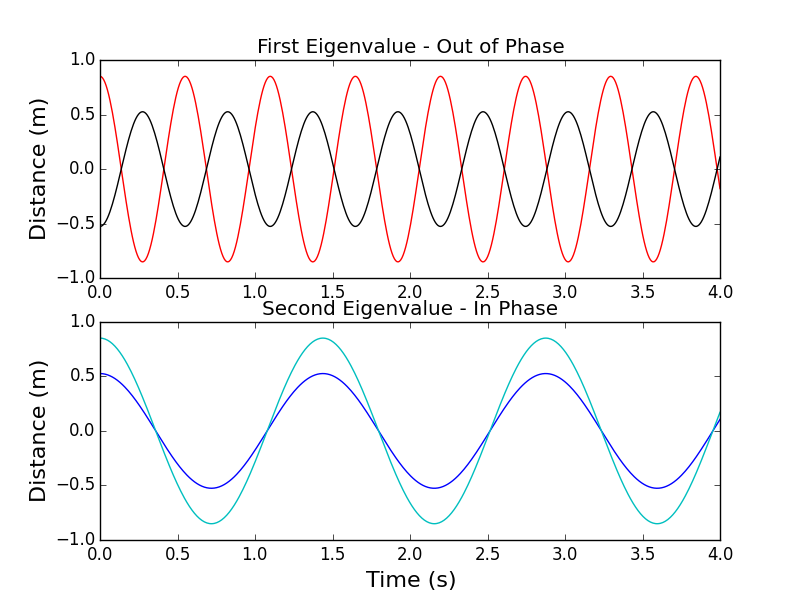
\includegraphics[scale=.45]{fig.png}
\end{figure}
\section{Code}

\begin{verbatim}
#Colt Bradley
#3.1.16
#Lesson 13 Homeowkr

#import modules
import numpy as n
import pylab as p

#define values
k = 15.
m = .3

#define matrix, solve
mat = n.matrix([[2*k,-k],[-k,k]])
eval, evec = n.linalg.eig(mat)

#redefine eigenvalues as omega
omeg = n.sqrt(eval/m)

#create times, build lists of function values for each time
t = n.linspace(0,4,500)
eig1_1 = evec[0,0]*n.cos(omeg[0]*t)
eig1_2 = evec[1,0]*n.cos(omeg[0]*t)
eig2_1 = evec[0,1]*n.cos(omeg[1]*t) 
eig2_2 = evec[1,1]*n.cos(omeg[1]*t)

#plot on the same plot using subplots and appropriate labeling. 
p.subplot(211)
p.title("First Eigenvalue - Out of Phase")
p.ylabel("Distance (m)",fontsize = 16)
p.plot(t,eig1_1,"r",label = "Eig1_1")
p.plot(t,eig1_2,"k",label = "Eig1_2")

p.subplot(212)
p.title("Second Eigenvalue - In Phase")
p.plot(t,eig2_1,"b", label = "Eig2_1")
p.plot(t,eig2_2,"c",label = "Eig2_2")
p.ylabel("Distance (m)",fontsize = 16)
p.xlabel("Time (s)",fontsize = 16)
p.show()
p.savefig("fig.png")
\end{verbatim}


\end{document}